\chapter{Data quality monitoring through trigger efficiencies }

\textbf{NOTE: You must explain DAQ chain and Tier0 before this section! Also offline reconstruction.}

The ATLAS detector is neither perfect nor constant in it's opperation and performance. Conditions change, components fail, some parts of the detector even move on occasion. In order to effectively and accurately measure anything at all, the detector must be well understood, calibrated and recalibrated on an almost weekly basis. The understanding of the detector performance is achieved through the data quality monitoring (DQM) group; differentially in terms of sub-detectors and physis signatures. 

An exhaustive description of the entire DQM chain is not practical, however the process can be roughly simplified into three stages; Online monitoring which occurs as the data is taken, by experts in the ATLAS control room (ACR), and Offline monitoring which occurs run by run within 24 hours of a run's completion. The data quality is also periodically reassessed each time a large data period is reprocessed with improved software. 

Online monitoring must be fast and as a consequence quite simple. For sub-detector DQM, for example the SCT, this may involve checking that the voltage bias is stable and that no individual modules are malfunctioning. For trigger, for example trigger tracking, this may involve checking that the distribution of tracks in $\eta$ and $\phi$ are as expected. 

Offline monitoring has, in theory, no time limit. However if a problem is found it is important to identify and correct it as soon as possible and for this reason the offline DQM for a particular run usually occurs within 24 hours of the data being taken. Because of the relaxed time constraints, offline monitoring can be more rigarous and each sub-detector and physics group has developed numerous batteries of tests and procdures to identify problems efficiently and in short time.

Trigger efficiencies can be sub-divided into two basic types; Absolute monitoring and relative monitoring. Absolute monitoring measures parameters and performance that directly correlates to the performance of the detector. An example would be checking that trigger jets were not found in one particular region of the detector more than others, or that trigger algorithms performed within their time restrictions and did not cause backflow in the DAQ chain. Relative monitoring measures parameters with respect to some other more ideal parameters. An example would be to compare trigger electrons properties to electrons reconstructed by the offline software at Tier0. Absolute efficiencies are useful for measuring performance of particular sub-detecotrs, whereas relative efficiencies are well suited to monitoring performance of trigger reconstruction algorithms.

\section{Regions of interest}
Triggers at the LHC create regions of interest (ROIs). At L1, an event may be selected with a large amount of jet activity in certain regions of the detector. These regions are identified as ROIs and passed to L2, where the trigger algorithms will execute on all detector information in this region and reconstruct detector objects such as inner detector tracks and calorimeter clusters. This is crucial to efficient trigger opperation. Many of the reconstruction algorithms are CPU intensive and it would not be possible to run them on the entire detector for each event triggered at L1 and maintian the required trigger rates. ROIs identify the intersting regions of the detector, reducing the regions on which the reconstruction algorithms must opperate. Occasionally the detector is run in ``full scan'' mode where these algorithms run on the entire detector for the purposes of unbiased measurements and performance monitoring.

%\section{Data quality slices}

%Monitoring of data quality is subdivided into groups or 'slices'. Each sub-detector has it's own slice, such as Pixel, SCT, etc and each physics signature also has it's own slice, such as EGamma, BJets and Muons. There is also a third group of slices that monitor detector objects that are used to construct physics signatures, such as ID tracking and Calorimeter Jets. Each slice is unique with it's own techniques and problems. In this thesis the trigger tracking will be described in detail. 

\section{Trigger Tracking}
\label{sec:tracks}

\begin{itemize}
\item What tracking information is availible at L2 and EF?
\item Why is it important to optimize execution time?
\item Why is it important to monitor performance.
\item Mention that there is more than one way to reconstruct tracks and that this often involves some physical motivation such as what signature you're looking for or what part of the ID you want to use.
\end{itemize}

At L1, trigger tracking is not possible. The ID is so taxing on the DAQ system that it would not be possible to read out the detectors and make any useful decision using hardware alone. Following the inclusion of the insertible b-layer and the second LHC run, some rudimentary tracking information will be availible before trigger L2. Since this information was not availible in the 2011 or 2012 data runs it will not be discussed further. 

At L2, read out of the inner detector is possible and trigger tracks are reconstructed. There are still strict time constraints but it is possible to reconstruct tracks and provide these for other signatures to use in their trigger decisions, such as tracks for electrons for egamma triggers.

At EF the time restrictions are more generous, and tracking almost as effecitve as that used in offline reconstruction is possible. It is very rare for a tracking algorithm to exceed it's permitted execution time, called a 'time out' at either L2 or EF and they are so few that each occurance is investigated individually.

Many phyiscs objects use inner detector trigger tracks in some form. All charged lepton signatures use the ID tracks (though muons may be reconstructed without them) as well as b-jet signatures and b-physics signatures and it is important to optimise the performance for each through the use of multiple track reconstruction algorithms. The signatures that use inner detector tracks, and the algorithms they use are listed in Table~\ref{tab:trig_tracks} and described in section~\ref{sec:tracks}.

\begin{table}
	\begin{center}
	\begin{tabular}{c c c c }
	\hline
	Signature & Uses ID Tracks & Primary Algorithm 2011 &  Primary Algorithm 2012 \\
	\hline
	Electron  & Yes & IDScan & L2Star-A \\
	Photon    & No  & - & - \\      
	Muon      & Yes & IDScan & L2Star-A \\
	Tau         & Yes & SiTrack & L2Star-B \\
	MET        & No & - & - \\
	Jet          & No & - & - \\
	B-Jet       & Yes & SiTrack & L2Star-B \\
	BPhys     & Yes & SiTrack & L2Star-B \\
	\hline
	\end{tabular}
	\end{center}
	\caption{Trigger signatures and their associated tracking algorithms in 2011 and 2012.}
	\label{tab:trig_tracks}
\end{table}

\subsection{Trigger Tracking Algorithms}

\subsubsection*{IDScan}
The IDScan (\emph{``Inner Detector Scan"}) algorithm is a L2 tracking algorithm optimised for tracks originating from a primary vertex. It is comprised of four sub-algorithms; the Z Finder, Hit Filter, Group Cleaner and Track Fitter. The Z Finder determines the z position of the primary vertex by extrapolating pairs of space points back to the z axis and locating the most densely populated region. The Hit Filter then groups space points compatible with track coming from this z region in $\eta$-$\phi$ space. The Group Cleaner then splits these groups into tracks and removes hits coming from noise. Each triplet of hits may now form a potential track from which their $p_T$,$\phi_0$ and $d_0$ may be measured. These triplets are then grouped based on similar $p_T$,$\phi_0$ and $d_0$ values and is accepted as a track of the group contains enough hits. The Track Fitter then calculates track parameters using a Kalman fitter~\cite{Gaines:2000qc,Candlin:2001fa}. 

The IDScan algorithm is well suited to reconstructing tracks originating from the primary vertex and is used as the primary L2 trigger algorithm for electron and muon signaturs.

\subsubsection*{SiTrack}
SiTrack (\emph{``Silicon Tracker"}) is an algorithm that also opperates at L2 however unlike IDScan, it is optimised to finding tracks from displaced vertices rather than those originating from the primary vertex. Rather than having a linear sub-algorithm execution structure, SiTrack has configurable pattern recognition modules. In many cases these overlap with functions available in IDScan (track fitting is very similar) however SiTrack uses blah blahg blah.

\subsubsection*{L2Star A, B and C}
The IDScan and SiTrack algorithms have significant 

\subsubsection*{EFID}
The EFID (\emph{``Event Filter Inner Detector"}) algorithm is similar in execution to the offline track reconstruction.


%\subsection{Inside-Out Algorithms}

%Inside-out algorithms reconstruct tracks starting from the pixel detector and moving outwards into the SCT and TRT detectors. These algorithms are ideal for reconstructing tracks coming from prompt signatures such as leptons from Z-boson decays. Tracks are seeded from a central z region and space points are blah blah blah. In 2011 data this was accomplished by the Inner Detector Scan (IDScan) algorithm at L2. In 2012 data, the ``A" instance of the L2Star algorithm is used. 

%What does EF do?

%\begin{itemize}
%\item What is Inside-out?
%\item What sort of signatures is this better for?
%\item IDTrack, the L2 2011 inside-out algorithm.
%\item L2StarA, the L2 2012 inside-out algorithm.
%\item EF tracking 
%\end{itemize}

%\subsection{Outside-In Algorithms}

%Outside-in algorithms reconstruct tracks starting from the SCT and moving into the Pixel detector. These algorithms reconstruct pairs of space points and then tracks, and as such are not as restricted to tracks pointing directly to the interaction point. This makes these algorithms ideal for trigger tracks arrising from displaced vertices, such as from b-jets or tau decays.
%In 2011 this tracking was accomplished at L2 by the Silicon Tracking (SiTrack) algorithm. In 2012 the ``B'' instance of the L2Star algorithm is used.

%\begin{itemize}
%\item What is Outside-in?
%\item What sort of signatures is this better for?
%\item SiTrack, the 2011 inside-out algorithm.
%\item L2StarB, the 2012 inside-out algorithm.
%\item EF tracking 
%\item Tracking using the TRT detector.
%\end{itemize}

\subsection{Relative Efficiency Monitoring}

The measurement of an efficiency requires some known quantity to use as a reference.  There are a number of physical objects available that suit this purpose. We may use other measurements that we expect to be reasonably good, for example the offline tracking algorithms where there are no execution time constraints (\emph{``relative efficiency")} or to some standard candle physical process such as Z boson production (\emph{``absolute efficiency")}.

The simplest relative effiicency is to compare all tracks inside an ROI that were reconstructed by the offline algorithms to those reconstructed by the trigger algorithms. In this case the deffinition of inefficient would be where a track was reconstructed buy the offline algorithms but was not reconstructed by the trigger algorithms. Conversely it is also possible to define a ``fake" efficiency, whereby a track that was reconstructed by the trigger algorithms but not by the offline algorithms is deemed to be a fake and constitutes a fake efficiency. 
The advantage of this technique is that it offers the possibility of high statistics, since more than one track can be reconstructed inside an ROI. This is not a trivial consideration. In order to measure trigger tracking efficiency, we require triggers that did not base their decision on any tracking infomation. Bandwidth for specialised triggers such as these is limited and it is difficult to obtain enough statistics to make useful assessments of efficiencies and hence data quality on a run by run basis.
The limitation of this technique is that many of the tracks that are reconstructed are not associated with a well defined or interesing physics object, and so a measurement of this efficiency does not have a well defined interpretation for physics analysis data quality. Nevertheless this technique is well suited for general detector opperation related data quality.

A more robust relative efficiency can be obtained by comparing to offline tracks that are associated with a physics object (\emph{``combined efficiency"}), for example a high $pT$ lepton. Such an measurement directly reflects the efficiency on which we trigger interesting physics objects, and clearly we would like this to be as high as possible. 
The limitation of this technique is that only one or at most two tracks in an ROI are usually associated with a physics object and so it is more statistically limited that other methods. This technique was introduced incrementally in 2011 running and results are only available for later runs for electron and tau signatures. No combined efficiencies we implemetned for b-jet triggers.

\subsection{Relative efficiencies in 2011 data}

During the 2011 ATLAS run, trigger tracking efficiencies were monitored on a run by run basis for electron, muon, tau and b-jet signatures for the IDScan, SiTrack and EFID algorithms.

\subsubsection*{Electrons}
Electron efficiencies were measured using two triggers. For earlier data periods efficiencies were measured using the ``e20 medium IDTrkNoCut trigger". In later data periods pileup conditions required the introduction of a tighter trigger that introduced additional isolation requirements ``e22vh medium IDTrkNoCut". 
Three example runs are shown in Fig.~\ref{fig:trig_2011_L2_pt_a} and Fig.~\ref{fig:trig_2011_EF_pt_a} corresponding to high statistics runs throughout the year. At L2 the ROI based effiicency of the IDScan algorithm remained stable at approximately 80\% with a fake rate of 10\%. The fake rate showed a strong dependence on track $\eta$. At EF the efficiency was stable at approximately 95\% with a fake efficiency of 5\%. 
The object based efficiencies were only implemented towards the end of the year and are only availible for the e22vh medium trigger. These showed an efficiency of 95\% for IDScan and 98\% for EFID.

\subsubsection*{Muons}
Muon efficiencies were measured using the ``mu20 IDTrkNoCut" trigger. Three example runs are shown in Fig.~\ref{fig:trig_2011_L2_pt_c} and Fig.~\ref{fig:trig_2011_EF_pt_c} corresponding to high statistics runs throughout the year. At L2 the ROI based effiicency of the IDScan algorithm remained stable at approximately 82\% with a fake rate of 5\%. The fake rate showed a dependence on track $\eta$ and was higher for low $p_T$ tracks. At EF the efficiency was stable at approximately 98\% with a fake efficiency of 4\%. 
The object based efficiencies showed an efficiency of 98\% for IDScan and over 99\% for EFID.

\subsubsection*{Taus}

\subsubsection*{B-Jets}

\subsubsection{Efficiencies in 2012 data}

\clearpage

\begin{figure}[htbp]
	\begin{subfigure}{.5\linewidth}
		\centering
		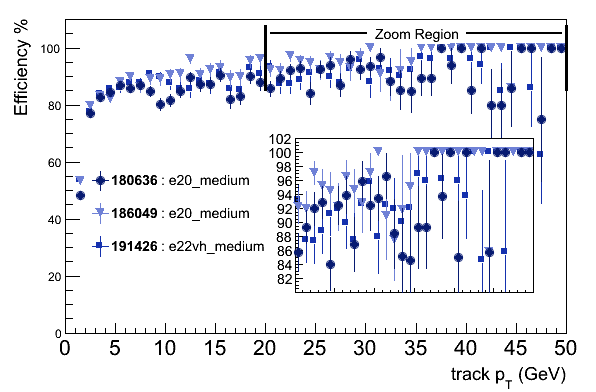
\includegraphics[width=75mm]{f/e20_medium_IDTrkNoCut_pT_IDS_eff}
		\caption{ROI based electron efficiencies.}
		\label{fig:trig_2011_L2_pt_a}
	\end{subfigure}
	\begin{subfigure}{.5\linewidth}	
		\centering
		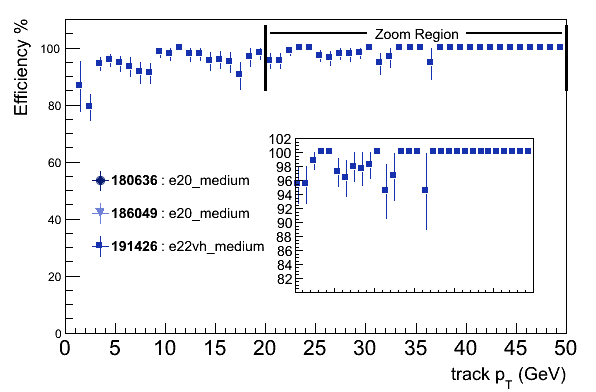
\includegraphics[width=75mm]{f/e20_medium_IDTrkNoCut_pT_IDS_eff_comb}
		\caption{Physics object based electron efficiencies.}
		\label{fig:trig_2011_L2_pt_b}
	\end{subfigure}
	\begin{subfigure}{.5\linewidth}	
		\centering
		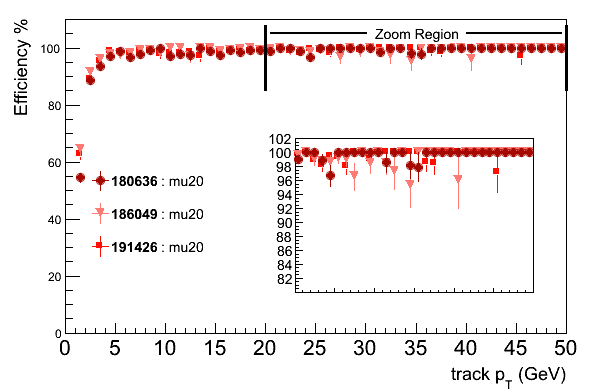
\includegraphics[width=75mm]{f/mu20_IDTrkNoCut_pT_IDS_eff}
		\caption{ROI based muon efficiencies.}
		\label{fig:trig_2011_L2_pt_c}
	\end{subfigure}
	\begin{subfigure}{.5\linewidth}	
		\centering
		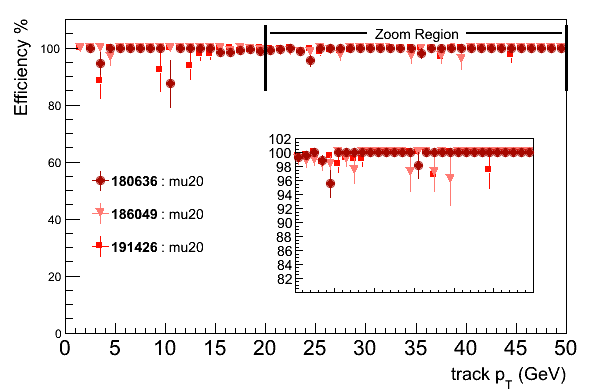
\includegraphics[width=75mm]{f/mu20_IDTrkNoCut_pT_IDS_eff_comb}
		\caption{Physics object based muon efficiencies.}
		\label{fig:trig_2011_L2_pt_d}
	\end{subfigure}
	\begin{subfigure}{.5\linewidth}	
		\centering
		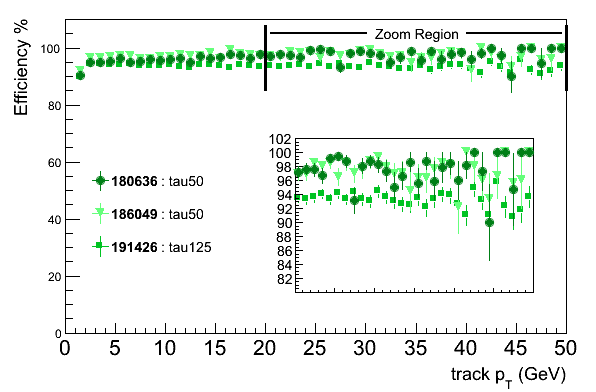
\includegraphics[width=75mm]{f/tau50_IDTrkNoCut_pT_SIT_eff}
		\caption{ROI based tau efficiencies.}
		\label{fig:trig_2011_L2_pt_e}
	\end{subfigure}
	\begin{subfigure}{.5\linewidth}	
		\centering
		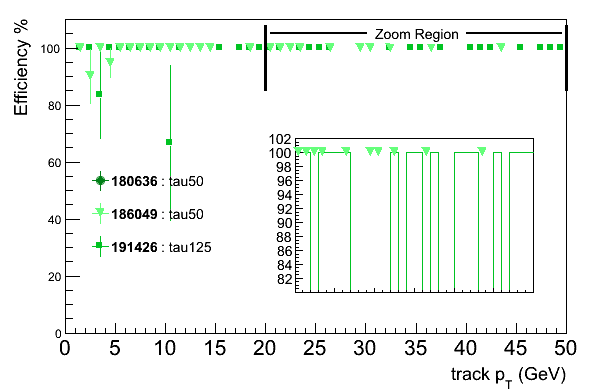
\includegraphics[width=75mm]{f/tau50_IDTrkNoCut_pT_SIT_eff_comb}
		\caption{Physics object based tau efficiencies.}
		\label{fig:trig_2011_L2_pt_f}
	\end{subfigure}
	\begin{center}
	\begin{subfigure}{.5\linewidth}	
		\centering
		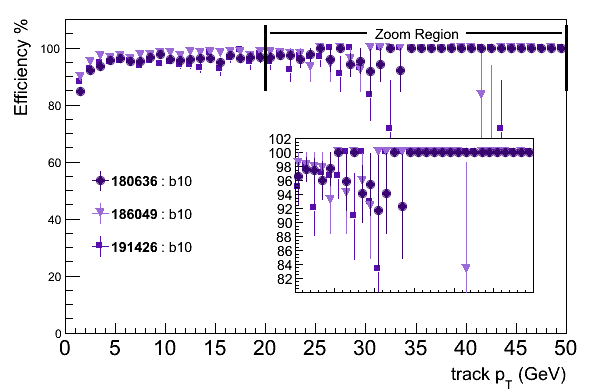
\includegraphics[width=75mm]{f/b10_IDTrkNoCut_pT_SIT_eff}
		\caption{ROI based b-jet efficiencies.}
		\label{fig:trig_2011_L2_pt_g}
	\end{subfigure}
	\end{center}
	\caption{Efficiencies of various L2 triggers for three high statistics runs in ATLAS 2011 data.}
	\label{fig:trig_2011_L2_pt}
\end{figure}

\clearpage

\begin{figure}[htbp]
	\begin{subfigure}{.5\linewidth}
		\centering
		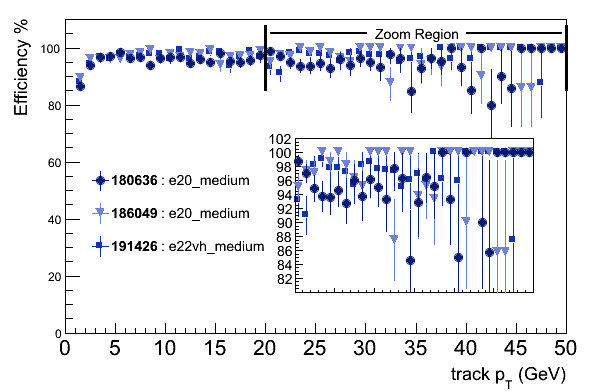
\includegraphics[width=75mm]{f/e20_medium_IDTrkNoCut_pT_EF_eff}
		\caption{ROI based electron efficiencies.}
		\label{fig:trig_2011_EF_pt_a}
	\end{subfigure}
	\begin{subfigure}{.5\linewidth}	
		\centering
		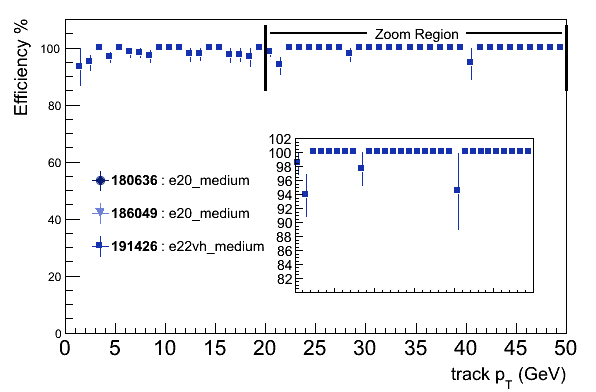
\includegraphics[width=75mm]{f/e20_medium_IDTrkNoCut_pT_EF_eff_comb}
		\caption{Physics object based electron efficiencies.}
		\label{fig:trig_2011_EF_pt_b}
	\end{subfigure}
	\begin{subfigure}{.5\linewidth}	
		\centering
		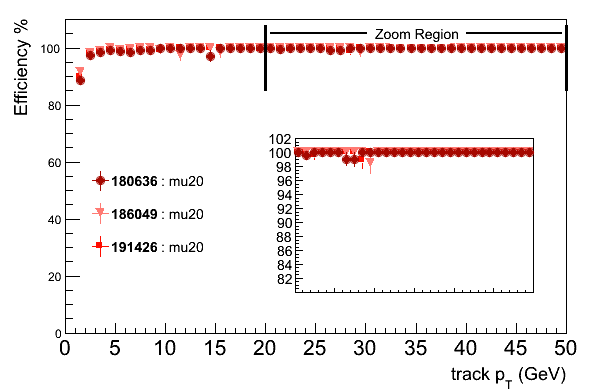
\includegraphics[width=75mm]{f/mu20_IDTrkNoCut_pT_EF_eff}
		\caption{ROI based muon efficiencies.}
		\label{fig:trig_2011_EF_pt_c}
	\end{subfigure}
	\begin{subfigure}{.5\linewidth}	
		\centering
		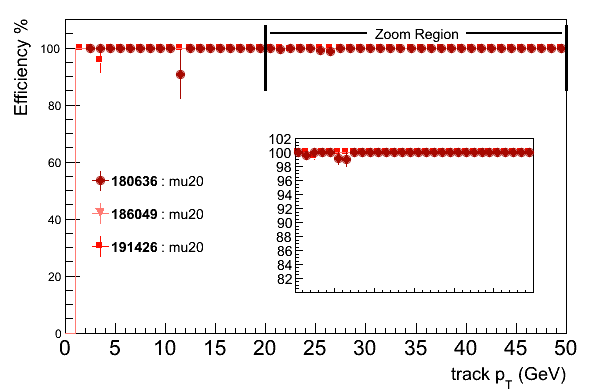
\includegraphics[width=75mm]{f/mu20_IDTrkNoCut_pT_EF_eff_comb}
		\caption{Physics object based muon efficiencies.}
		\label{fig:trig_2011_EF_pt_d}
	\end{subfigure}
	\begin{subfigure}{.5\linewidth}	
		\centering
		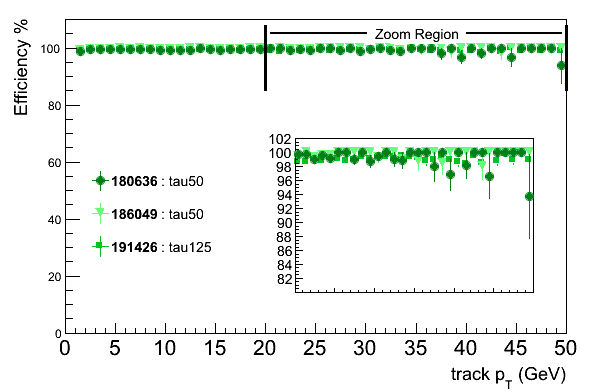
\includegraphics[width=75mm]{f/tau50_IDTrkNoCut_pT_EF_eff}
		\caption{ROI based tau efficiencies.}
		\label{fig:trig_2011_EF_pt_e}
	\end{subfigure}
	\begin{subfigure}{.5\linewidth}	
		\centering
		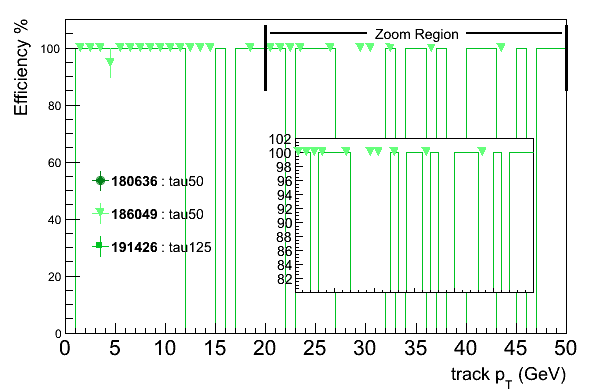
\includegraphics[width=75mm]{f/tau50_IDTrkNoCut_pT_EF_eff_comb}
		\caption{Physics object based tau efficiencies.}
		\label{fig:trig_2011_EF_pt_f}
	\end{subfigure}
	\begin{center}
	\begin{subfigure}{.5\linewidth}	
		\centering
		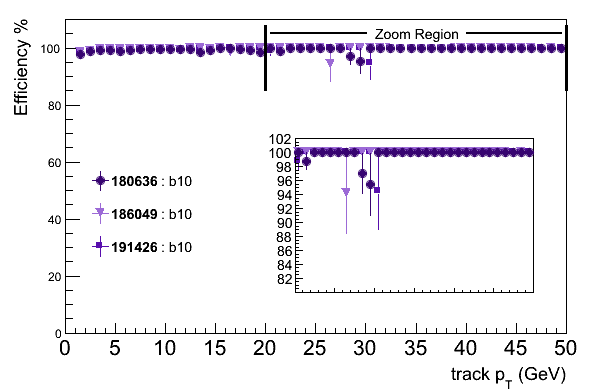
\includegraphics[width=75mm]{f/b10_IDTrkNoCut_pT_EF_eff}
		\caption{ROI based b-jet efficiencies.}
		\label{fig:trig_2011_EF_pt_g}
	\end{subfigure}
	\end{center}
	\caption{Efficiencies of various EF triggers for three high statistics runs in ATLAS 2011 data.}
	\label{fig:trig_2011_EF_pt}
\end{figure}

\clearpage

\begin{figure}[htbp]
	\begin{subfigure}{.5\linewidth}
		\centering
		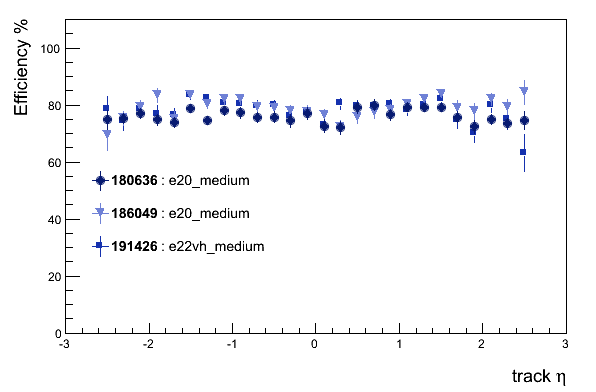
\includegraphics[width=75mm]{f/e20_medium_IDTrkNoCut_eta_IDS_eff}
		\caption{ROI based electron efficiencies.}
		\label{fig:trig_2011_L2_eta_a}
	\end{subfigure}
	\begin{subfigure}{.5\linewidth}	
		\centering
		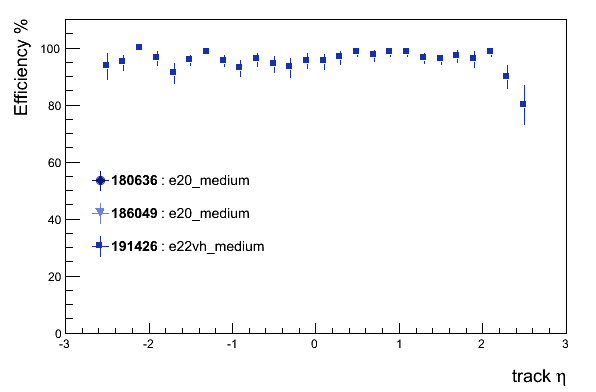
\includegraphics[width=75mm]{f/e20_medium_IDTrkNoCut_eta_IDS_eff_comb}
		\caption{Physics object based electron efficiencies.}
		\label{fig:trig_2011_L2_eta_b}
	\end{subfigure}
	\begin{subfigure}{.5\linewidth}	
		\centering
		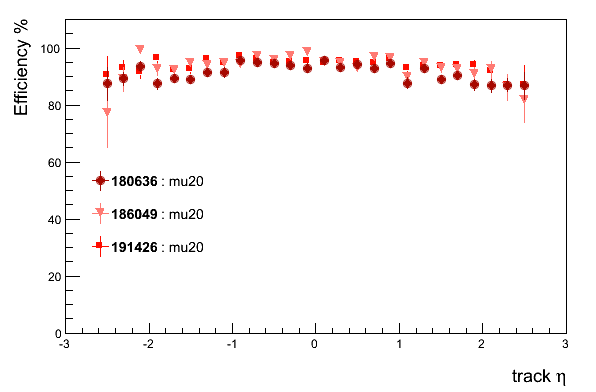
\includegraphics[width=75mm]{f/mu20_IDTrkNoCut_eta_IDS_eff}
		\caption{ROI based muon efficiencies.}
		\label{fig:trig_2011_L2_eta_c}
	\end{subfigure}
	\begin{subfigure}{.5\linewidth}	
		\centering
		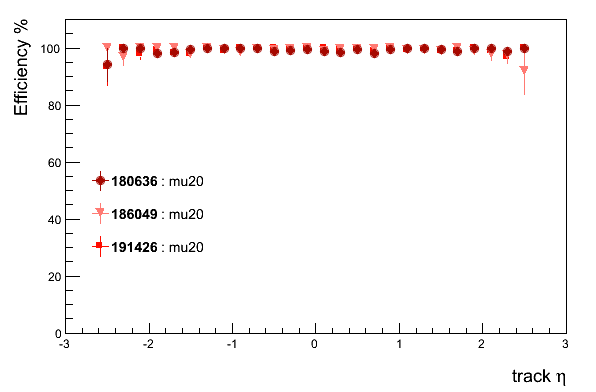
\includegraphics[width=75mm]{f/mu20_IDTrkNoCut_eta_IDS_eff_comb}
		\caption{Physics object based muon efficiencies.}
		\label{fig:trig_2011_L2_eta_d}
	\end{subfigure}
	\begin{subfigure}{.5\linewidth}	
		\centering
		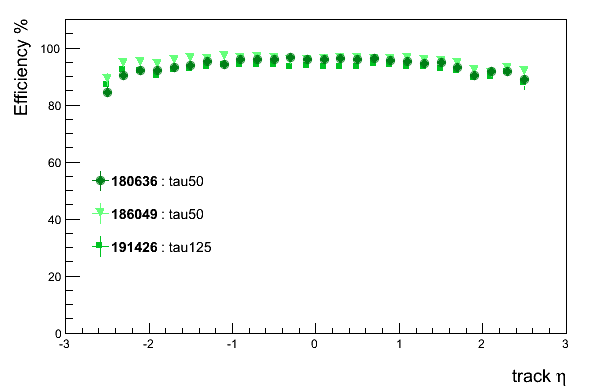
\includegraphics[width=75mm]{f/tau50_IDTrkNoCut_eta_SIT_eff}
		\caption{ROI based tau efficiencies.}
		\label{fig:trig_2011_L2_eta_e}
	\end{subfigure}
	\begin{subfigure}{.5\linewidth}	
		\centering
		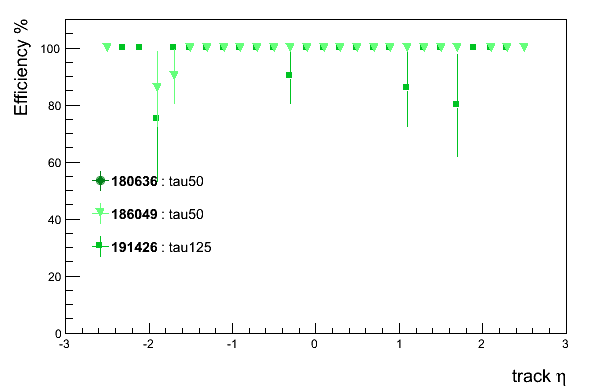
\includegraphics[width=75mm]{f/tau50_IDTrkNoCut_eta_SIT_eff_comb}
		\caption{Physics object based tau efficiencies.}
		\label{fig:trig_2011_L2_eta_f}
	\end{subfigure}
	\begin{center}
	\begin{subfigure}{.5\linewidth}	
		\centering
		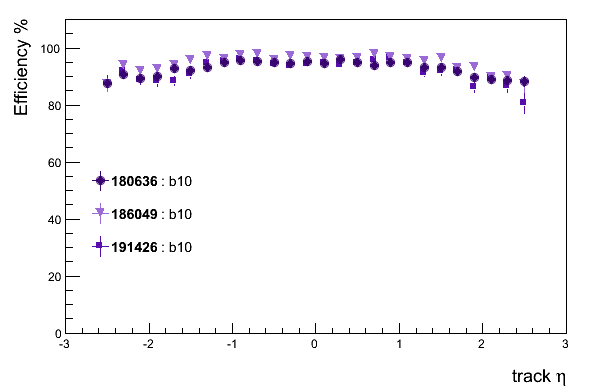
\includegraphics[width=75mm]{f/b10_IDTrkNoCut_eta_SIT_eff}
		\caption{ROI based b-jet efficiencies.}
		\label{fig:trig_2011_L2_eta_g}
	\end{subfigure}
	\end{center}
	\caption{Efficiencies of various L2 triggers for three high statistics runs in ATLAS 2011 data.}
	\label{fig:trig_2011_L2_eta}
\end{figure}

\clearpage

\begin{figure}[htbp]
	\begin{subfigure}{.5\linewidth}
		\centering
		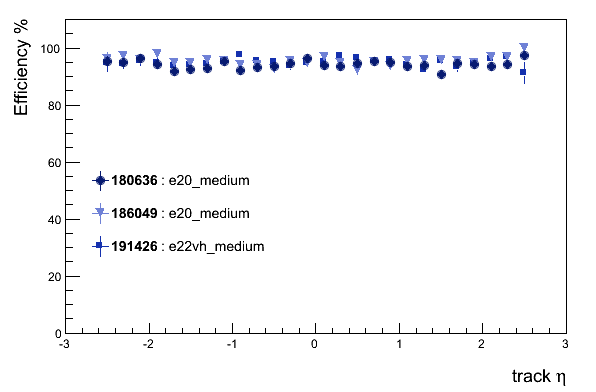
\includegraphics[width=75mm]{f/e20_medium_IDTrkNoCut_eta_EF_eff}
		\caption{ROI based electron efficiencies.}
		\label{fig:trig_2011_EF_eta_a}
	\end{subfigure}
	\begin{subfigure}{.5\linewidth}	
		\centering
		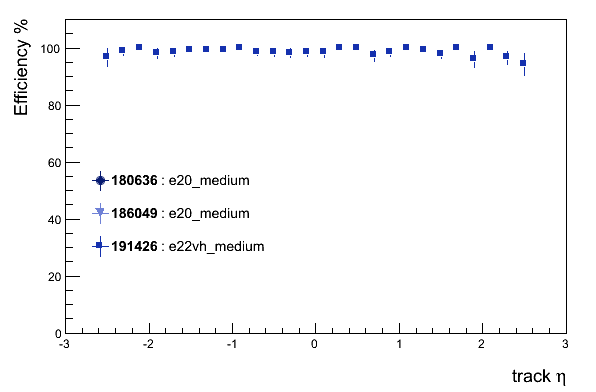
\includegraphics[width=75mm]{f/e20_medium_IDTrkNoCut_eta_EF_eff_comb}
		\caption{Physics object based electron efficiencies.}
		\label{fig:trig_2011_EF_eta_b}
	\end{subfigure}
	\begin{subfigure}{.5\linewidth}	
		\centering
		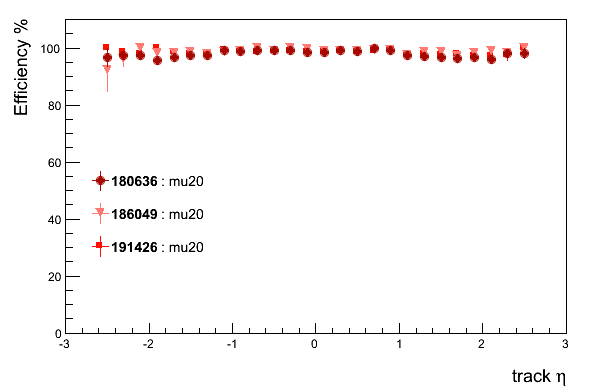
\includegraphics[width=75mm]{f/mu20_IDTrkNoCut_eta_EF_eff}
		\caption{ROI based muon efficiencies.}
		\label{fig:trig_2011_EF_eta_c}
	\end{subfigure}
	\begin{subfigure}{.5\linewidth}	
		\centering
		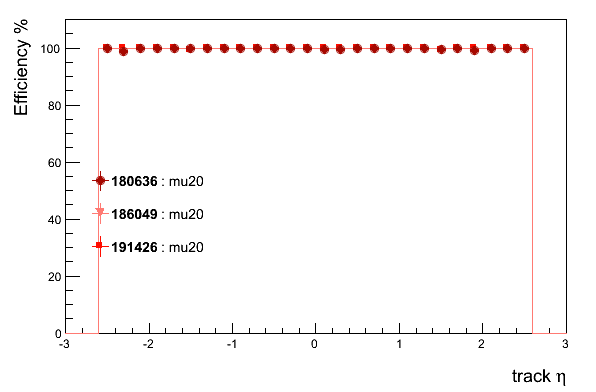
\includegraphics[width=75mm]{f/mu20_IDTrkNoCut_eta_EF_eff_comb}
		\caption{Physics object based muon efficiencies.}
		\label{fig:trig_2011_EF_eta_d}
	\end{subfigure}
	\begin{subfigure}{.5\linewidth}	
		\centering
		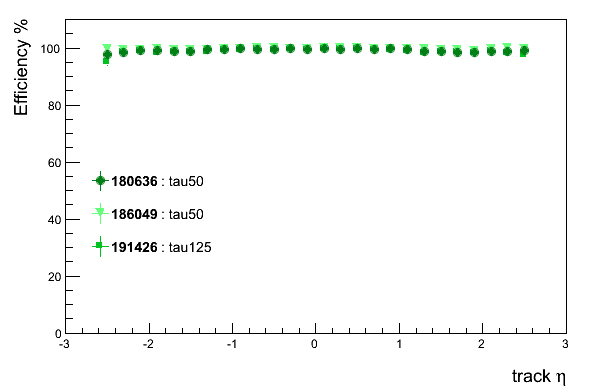
\includegraphics[width=75mm]{f/tau50_IDTrkNoCut_eta_EF_eff}
		\caption{ROI based tau efficiencies.}
		\label{fig:trig_2011_EF_eta_e}
	\end{subfigure}
	\begin{subfigure}{.5\linewidth}	
		\centering
		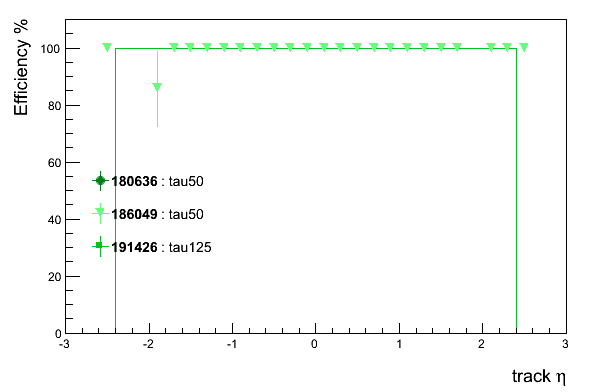
\includegraphics[width=75mm]{f/tau50_IDTrkNoCut_eta_EF_eff_comb}
		\caption{Physics object based tau efficiencies.}
		\label{fig:trig_2011_EF_eta_f}
	\end{subfigure}
	\begin{center}
	\begin{subfigure}{.5\linewidth}	
		\centering
		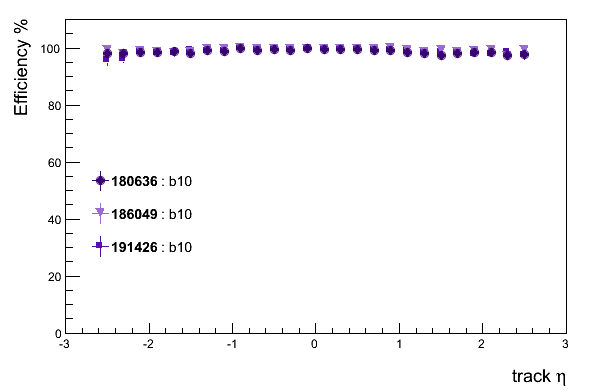
\includegraphics[width=75mm]{f/b10_IDTrkNoCut_eta_EF_eff}
		\caption{ROI based b-jet efficiencies.}
		\label{fig:trig_2011_EF_eta_g}
	\end{subfigure}
	\end{center}
	\caption{Efficiencies of various EF triggers for three high statistics runs in ATLAS 2011 data.}
	\label{fig:trig_2011_EF_eta}
\end{figure}

\clearpage

\begin{figure}[htbp]
	\begin{subfigure}{.5\linewidth}
		\centering
		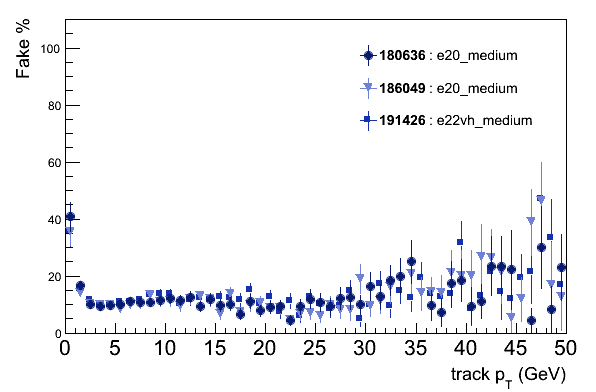
\includegraphics[width=75mm]{f/e20_medium_IDTrkNoCut_pT_IDS_fake}
		\caption{ROI based electron efficiencies.}
		\label{fig:trig_2011_L2_pt_a}
	\end{subfigure}
	\begin{subfigure}{.5\linewidth}	
		\centering
		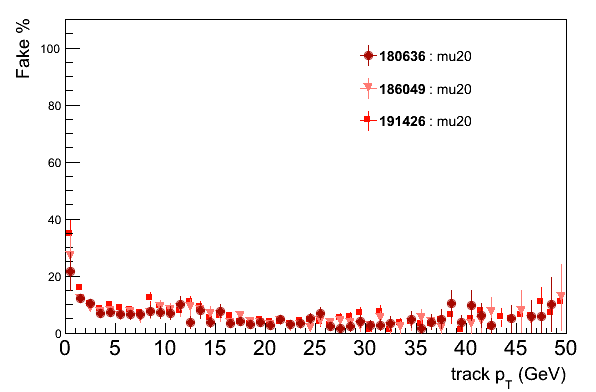
\includegraphics[width=75mm]{f/mu20_IDTrkNoCut_pT_IDS_fake}
		\caption{ROI based muon efficiencies.}
		\label{fig:trig_2011_L2_pt_c}
	\end{subfigure}
	\begin{subfigure}{.5\linewidth}	
		\centering
		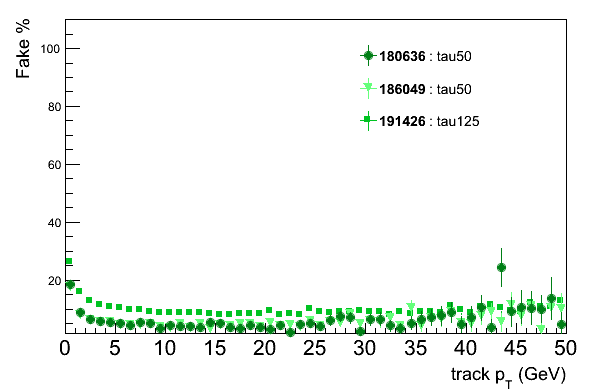
\includegraphics[width=75mm]{f/tau50_IDTrkNoCut_pT_SIT_fake}
		\caption{ROI based tau efficiencies.}
		\label{fig:trig_2011_L2_pt_e}
	\end{subfigure}
	\begin{subfigure}{.5\linewidth}	
		\centering
		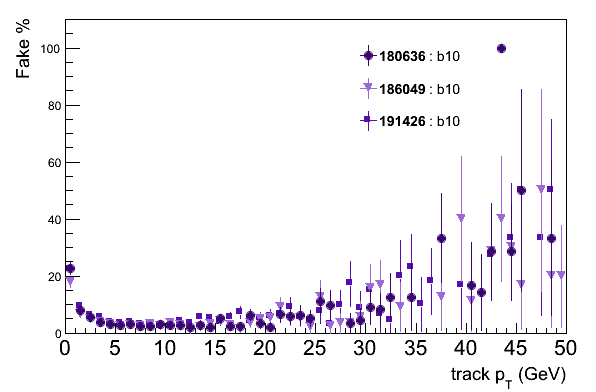
\includegraphics[width=75mm]{f/b10_IDTrkNoCut_pT_SIT_fake}
		\caption{ROI based b-jet efficiencies.}
		\label{fig:trig_2011_L2_pt_g}
	\end{subfigure}
	\caption{Efficiencies of various L2 triggers for three high statistics runs in ATLAS 2011 data.}
	\label{fig:trig_2011_L2_pt}
\end{figure}

\clearpage

\begin{figure}[htbp]
	\begin{subfigure}{.5\linewidth}
		\centering
		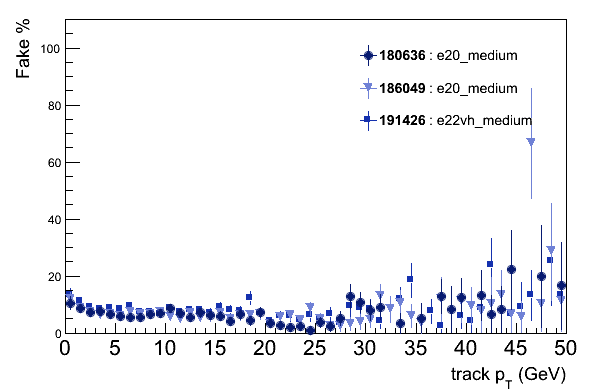
\includegraphics[width=75mm]{f/e20_medium_IDTrkNoCut_pT_EF_fake}
		\caption{ROI based electron efficiencies.}
		\label{fig:trig_2011_EF_pt_a}
	\end{subfigure}
	\begin{subfigure}{.5\linewidth}	
		\centering
		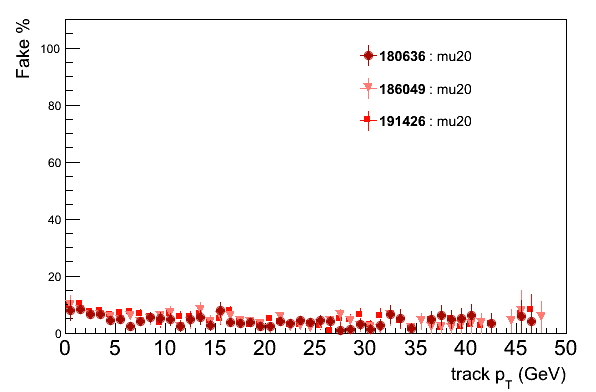
\includegraphics[width=75mm]{f/mu20_IDTrkNoCut_pT_EF_fake}
		\caption{ROI based muon efficiencies.}
		\label{fig:trig_2011_EF_pt_c}
	\end{subfigure}
	\begin{subfigure}{.5\linewidth}	
		\centering
		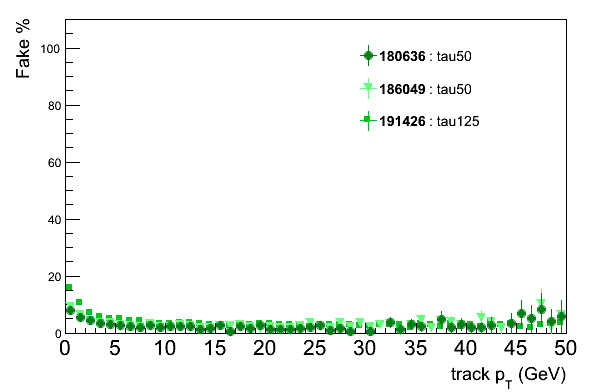
\includegraphics[width=75mm]{f/tau50_IDTrkNoCut_pT_EF_fake}
		\caption{ROI based tau efficiencies.}
		\label{fig:trig_2011_EF_pt_e}
	\end{subfigure}
	\begin{subfigure}{.5\linewidth}	
		\centering
		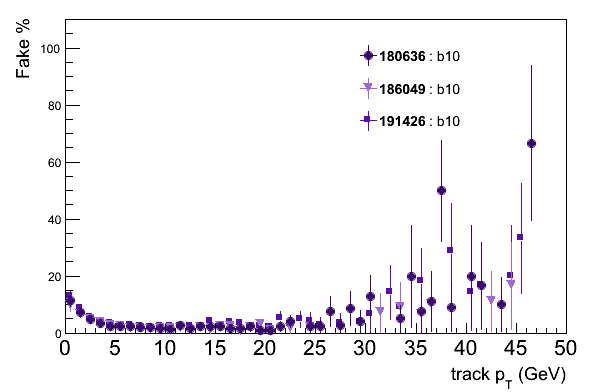
\includegraphics[width=75mm]{f/b10_IDTrkNoCut_pT_EF_fake}
		\caption{ROI based b-jet efficiencies.}
		\label{fig:trig_2011_EF_pt_g}
	\end{subfigure}
	\caption{Efficiencies of various EF triggers for three high statistics runs in ATLAS 2011 data.}
	\label{fig:trig_2011_EF_pt}
\end{figure}

\clearpage

\begin{figure}[htbp]
	\begin{subfigure}{.5\linewidth}
		\centering
		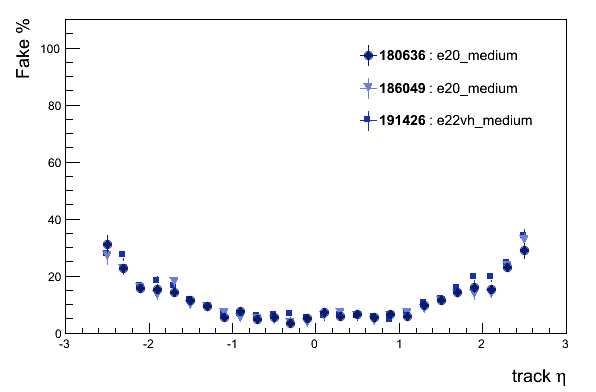
\includegraphics[width=75mm]{f/e20_medium_IDTrkNoCut_eta_IDS_fake}
		\caption{ROI based electron efficiencies.}
		\label{fig:trig_2011_L2_eta_a}
	\end{subfigure}
	\begin{subfigure}{.5\linewidth}	
		\centering
		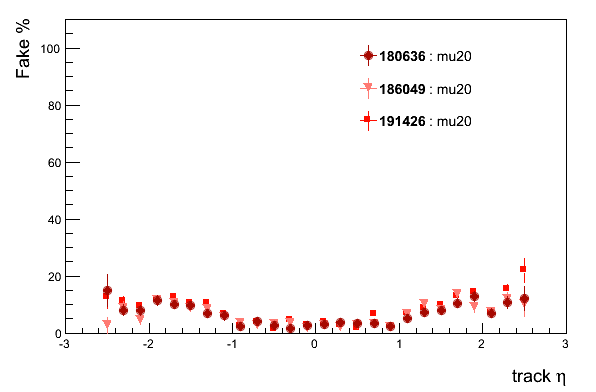
\includegraphics[width=75mm]{f/mu20_IDTrkNoCut_eta_IDS_fake}
		\caption{ROI based muon efficiencies.}
		\label{fig:trig_2011_L2_eta_c}
	\end{subfigure}
	\begin{subfigure}{.5\linewidth}	
		\centering
		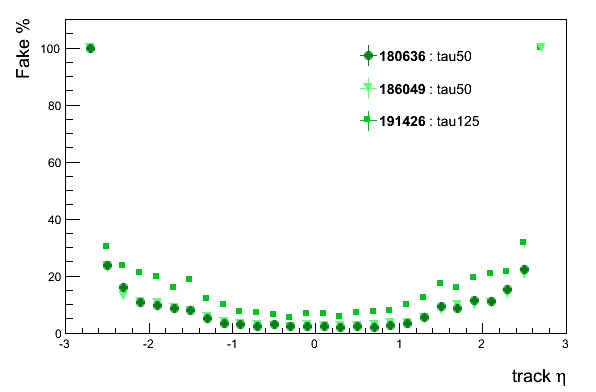
\includegraphics[width=75mm]{f/tau50_IDTrkNoCut_eta_SIT_fake}
		\caption{ROI based tau efficiencies.}
		\label{fig:trig_2011_L2_eta_e}
	\end{subfigure}
	\begin{subfigure}{.5\linewidth}	
		\centering
		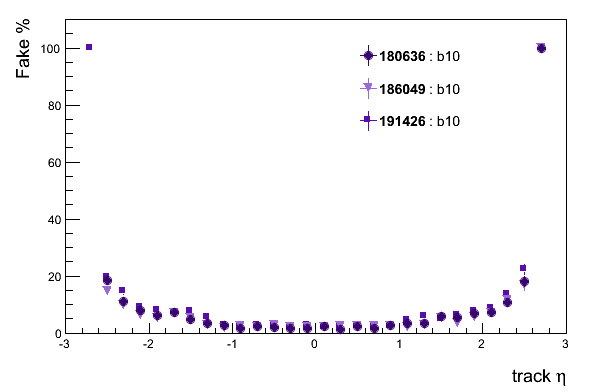
\includegraphics[width=75mm]{f/b10_IDTrkNoCut_eta_SIT_fake}
		\caption{ROI based b-jet efficiencies.}
		\label{fig:trig_2011_L2_eta_g}
	\end{subfigure}
	\caption{Efficiencies of various L2 triggers for three high statistics runs in ATLAS 2011 data.}
	\label{fig:trig_2011_L2_eta}
\end{figure}

\clearpage

\begin{figure}[htbp]
	\begin{subfigure}{.5\linewidth}
		\centering
		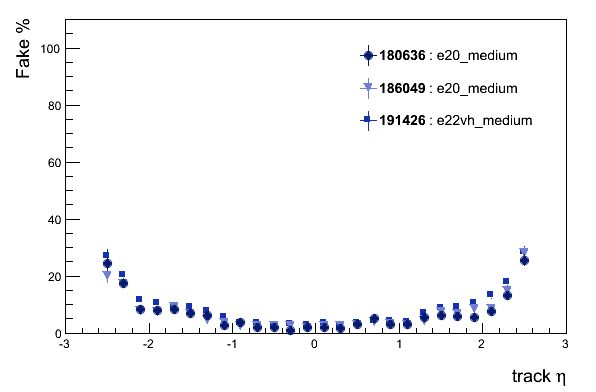
\includegraphics[width=75mm]{f/e20_medium_IDTrkNoCut_eta_EF_fake}
		\caption{ROI based electron efficiencies.}
		\label{fig:trig_2011_EF_eta_a}
	\end{subfigure}
	\begin{subfigure}{.5\linewidth}	
		\centering
		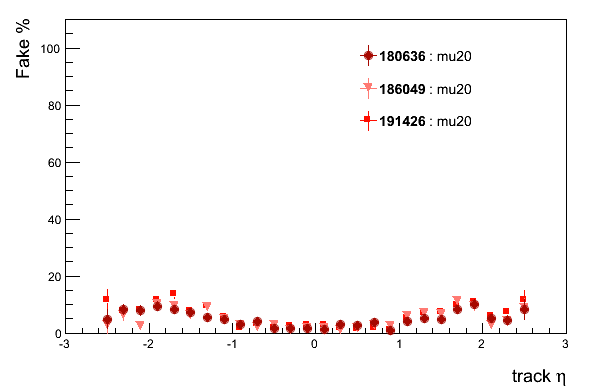
\includegraphics[width=75mm]{f/mu20_IDTrkNoCut_eta_EF_fake}
		\caption{ROI based muon efficiencies.}
		\label{fig:trig_2011_EF_eta_c}
	\end{subfigure}
	\begin{subfigure}{.5\linewidth}	
		\centering
		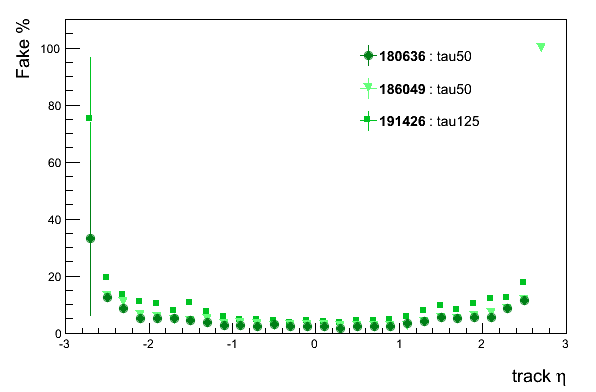
\includegraphics[width=75mm]{f/tau50_IDTrkNoCut_eta_EF_fake}
		\caption{ROI based tau efficiencies.}
		\label{fig:trig_2011_EF_eta_e}
	\end{subfigure}
	\begin{subfigure}{.5\linewidth}	
		\centering
		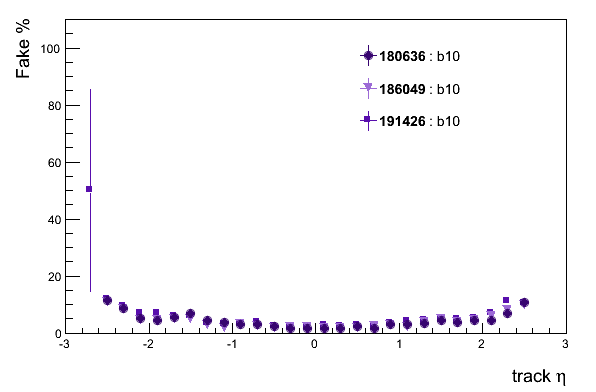
\includegraphics[width=75mm]{f/b10_IDTrkNoCut_eta_EF_fake}
		\caption{ROI based b-jet efficiencies.}
		\label{fig:trig_2011_EF_eta_g}
	\end{subfigure}
	\caption{Efficiencies of various EF triggers for three high statistics runs in ATLAS 2011 data.}
	\label{fig:trig_2011_EF_eta}
\end{figure}

\clearpage

\subsection{Absolute Efficiency Monitoring}

\begin{itemize}
\item Zee tag and probe motivation
\item Problems with bremstrahlung
\item Figure: Cartoon showing a brem with a track losing momentum but the electron and photon still going into the same calo cell.
\end{itemize}

\subsection{Software validation using tracking efficiencies}







